\section{Problema 1}

\subsection{Introducción}

Como primer acercamiento a este problema tratamos de buscar qué algoritmos de búsqueda de caminos vistos hasta el momento en la materia podían aplicarse al problema. Luego de pasar por varios nombres y tratar de forzar las características del problema para que pudieran aplicar, decidimos construir un algoritmo que resolviera el problema tratando de pensarlo desde el principio, y basándonos en ideas de 'BFS' y 'Kruskal'. Este último algoritmo era uno de los que en principio nos había parecido podía resolver el problema, pero luego lo descartamos a partir de encontrar distintos contraejemplos que mostraban la incorrecta aplicación a este problema.\\
\indent A continuación se presentan los pseudocódigos de los algoritmos, la demostración de correctitud con una explicación de la solución, el análisis del modelado de las estructuras y las complejidades de todas las funciones, y finalmente el análisis de la experimentación.

\subsection{Pseudocódigos}

\begin{algorithm}
\caption{buscarPeso (\textbf{in/out} mapa: \textsl{Mapa}) $\rightarrow$ res: \textsl{int}}
\begin{algorithmic}[1]

\STATE $heap \leftarrow$ crear heap de tramos vacío
\STATE estado $origen \leftarrow confirmado$
\STATE agregar tramos salientes de $origen$ al $heap$

\WHILE{estado $destino = no$ $confirmado$}
	\STATE $tramo \leftarrow$ pop elemento del $heap$
	\STATE $ciudad\_hasta \leftarrow$ ciudad a la que llega $tramo$
	\STATE $ciudad\_desde \leftarrow$ ciudad desde la que sale el $tramo$
	\IF{$estado$ $ciudad\_hasta = confirmado$} 
		\STATE continuar
	\ENDIF
	\STATE estado $ciudad\_hasta \leftarrow confirmado$
	\STATE peso $ciudad\_hasta \leftarrow min($peso $tramo$,peso $ciudad\_desde)$
	\STATE agregar tramos salientes de $ciudad$ al $heap$
	
\ENDWHILE
\RETURN peso $destino$  
\end{algorithmic}
\end{algorithm}

\begin{algorithm}
\caption{agregarTramos (\textbf{in/out} heap: \textsl{Heap}, \textbf{in} vecinos: \textsl{Lista(Tramo)}}
\begin{algorithmic}[1]

\WHILE{hay tramos en $vecinos$}
	\STATE sacar un $tramo$ de $vecinos$
	\STATE $ciudad\_hasta \leftarrow$ ciudad a la que llega el $tramo$
	\IF{estado $ciudad\_hasta$ = confirmado}
		\STATE no se agrega el $tramo$ al heap
	\ELSE 
		\STATE agregar $tramo$ al heap
	\ENDIF
\ENDWHILE
\end{algorithmic}
\end{algorithm}

\clearpage

\subsection{Demostración de Correctitud}

La idea de este algoritmo se apoya en un caso base, y luego en un caso general. El caso base consiste en mirar los tramos que salen desde la ciudad origen, tomar la que admite más peso y marcar como confirmada la ciudad a la que llega ese tramo, a la vez que se determina que ese es el máximo peso con el cual se puede llegar según las condiciones del problema. Esto es porque, si se hubiera salido por alguno de los otros caminos y se pudiera llegar a esa ciudad, seguro el cuello de botella hubiera sido menor que el peso de la arista elegida, el cual era el máximo. Luego se agregan en un heap los tramos que salen de esa ciudad confirmada, y se comienza un ciclo iterativo que termina sólo cuando la ciudad destino aparezca confirmada. Vale notar que el hecho de que una ciudad esté confirmada implica que no se vuelve a visitar, pues se ha ratificado que el peso que tiene asociado es el máximo con el que se puede llegar a esa ciudad desde el origen, dada las restricciones de los caminos.\\
\indent Durante la iteración de este ciclo se produce el caso general: del heap se toma la arista de peso máximo y se realiza el mismo procedimiento que antes, sólo aquí no se confirma a ciegas el peso con el que se puede llegar a la ciudad extremo de esa ruta, sino que se evalúa el mínimo entre el peso que tenía confirmado la ciudad fuente de esa arista y el peso de la misma.\\
\indent Dado que nunca se agrega dos veces una misma arista, y que no se vuelve a visitar una ciudad que ha sido confirmada, este proceso eventualmente confirma destino y termina. Para ver esto en lo que resta de la demostración, es necesario resaltar algunas propiedades del problema:

\begin{itemize}
	\item Como una característica del mapa es que el grafo subyacente sea
conexo, existe al menos un camino entre cualquier par de nodos, en particular entre las ciudades origen y destino.
	\item Durante el transcurso del ciclo iterativo se quita el elemento
más grande de un heap, y eso siempre se puede hacer porque el heap nunca está
vacío. Esto sucede porque una vez que una ciudad se confirma se agregan todos
sus caminos salientes al heap. En caso de llegar a una ciudad sin caminos
salientes, es porque pasa una de dos cosas: o bien es la ciudad destino, y el
algoritmo termina, o el último elemento quitado no era el único en el heap, ya
que todavía no se llegó a la ciudad destino, y el grafo es conexo.
\end{itemize}

\indent A continuación se exhibe un gráfico donde se muestran los distintos estados de una ejecución del algoritmo para un mapa pequeño. Para cada instancia puede observarse a la derecha de los mapas una tabla que representa el estado del heap. Se puede apreciar también cómo en cada iteración se extrae la ruta de peso máximo y se confirma el nodo al que llega dirimiendo entre el peso con el que se podía llegar a la ciudad anterior y el peso de la arista (para el caso general). En el extremo inferior derecho de la imagen puede observarse una tabla con el estado final del mapa y las pesos confirmados para cada ciudad.

\begin{figure}[h]
	\centering
	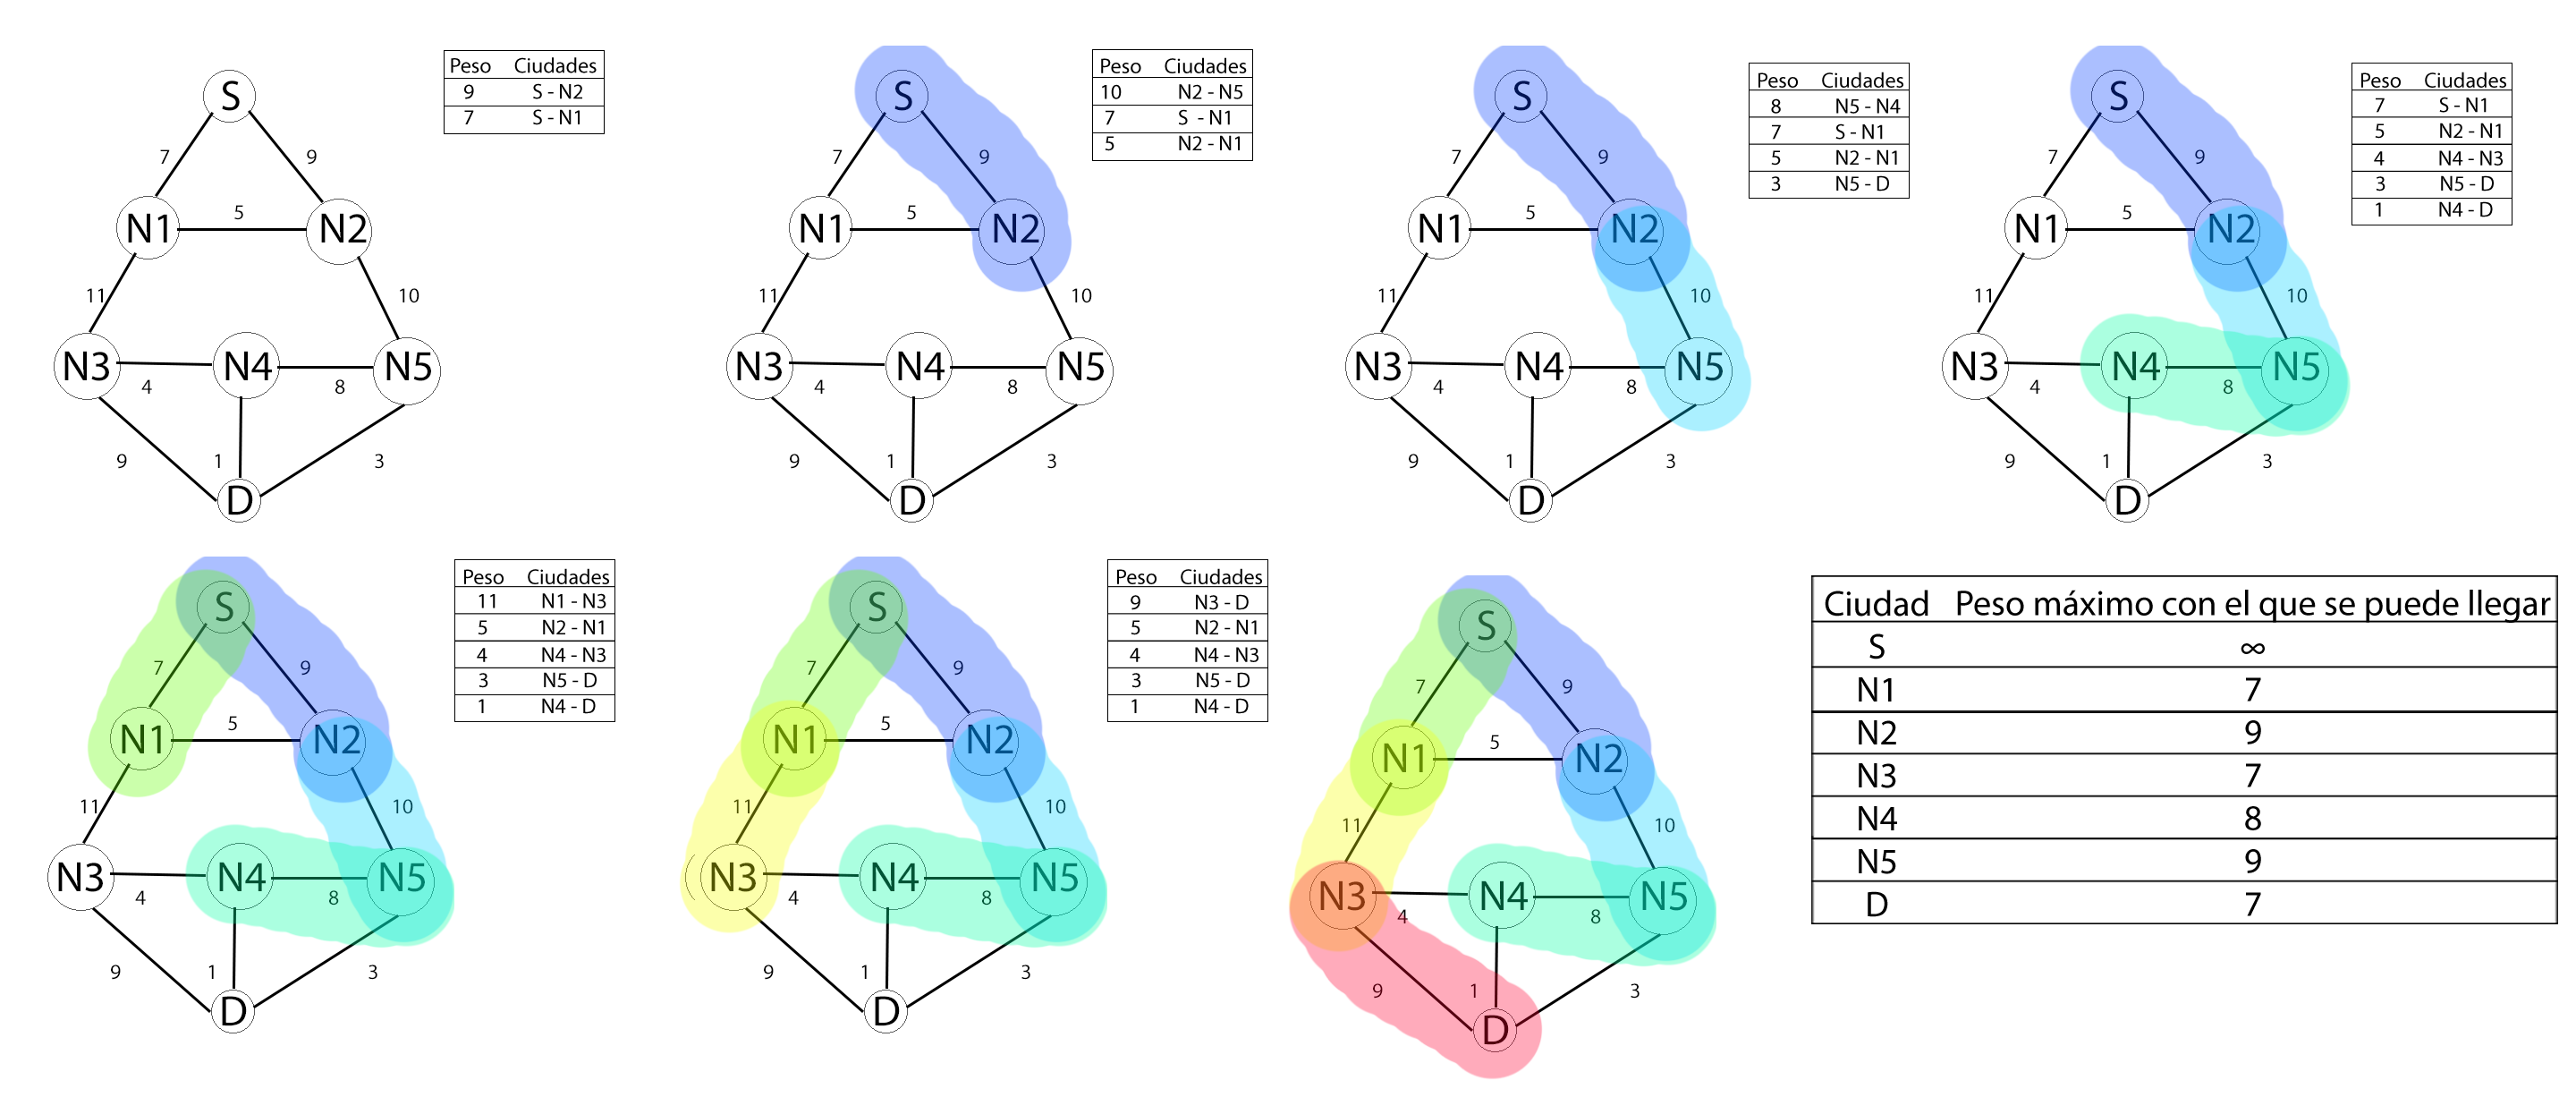
\includegraphics[width=450px]{./figs/algoritmoEj1.png}
\end{figure}

En un mapa dado viven varias ciudades conectadas por tramos. Estos se componen de un valor entero no negativo que indica el peso que pueden llevar, y dos ciudades que ofician como los extremos de la arista: desde dónde sale y hasta dónde llega. El
objetivo -de forma resumida- es llegar de la ciudad fuente a la ciudad destino
con el mayor peso posible, teniendo en cuenta que dado un camino, el peso máximo
con el que se puede llegar a destino, es el peso más chico dentro del conjunto
de pesos de las aristas que lo componen.\\
\indent Las ciudades tienen 2 estados (confirmado o no confirmado) y un campo peso. Lo que diferencian los estados es si la ciudad ya fue visitada o no. En el caso de haber sido visitada, su campo peso indica qué cantidad se puede trasladar desde el origen a ella, por lo que a una ciudad que ya fue confirmada no se le modificará dicho campo, ni su estado.\\
\indent La otra estructura importante utilizada es el heap, que ordena los tramos que se le agregan en función del peso que pueden trasladar, y pone en el tope a la de peso máximo. El heap además representa el conjunto de tramos que eventualmente se visitarán.\\
%\indent Al comenzar el algoritmo, se guardan todos los tramos desde los que se puede
%salir de la ciudad fuente en el heap. Se obtiene el de mayor peso, se le pone
%ese peso a la ciudad a la que va y se confirma la misma. Esta confirmación es
%correcta, ya que no puede pasar que se pueda llegar por otro camino con un peso
%mayor que el actual, ya que cualquiera de las otras aristas sale de origen con un peso menor, y eso ya un peor cuello de botella para llegar a esa ciudad. Una vez que se confirma la primera ciudad, se revisan los tramos que salen de la
%misma, y se agregan al heap. Se vuelve a obtener el tramo de mayor peso, y luego a la ciudad a la que va ese tramo, se le asigna el mínimo entre el peso de ese tramo y el peso actual que tiene, y se confirma la ciudad.\\
%\indent Este proceso se repite hasta que se encuentra la ciudad destino. Al llegar a la
%misma, va a haber un solo camino que va desde la ciudad fuente hasta la ciudad
%destino tal que dicho camino tenga todas las ciudades confirmadas, y
%posiblemente, otros caminos que se corten de forma prematura (porque en algún
%punto había un tramo que mejoraba todas las opciones que este camino tenía).
%(esto creo que es lo mismo que decir que hay aristas que nunca vamos a ver)

%// Creo que para la demo de correctitud habría que escribir esto un poco más
%formal, y justificar por que cada paso es el mejor de los pasos posibles, pero
%mucho más que formalizar un poco, ordenar las ideas y escribirlas no creo que
%necesitemos. Igual lo vemos.
\begin{itemize}
 \item \textbf{Caso Base} Veamos por qué la elección del primer paso es correcta con un poco más de detalle.\\
Supongamos que desde la ciudad fuente salen $n$ caminos.
Si tomamos el camino que puede soportar mas peso (lo llamamos p), podemos llegar
a la ciudad conectada por esta ruta (la llamamos $C_1$) con peso p. Ahora bien,
si hubiésemos tomado otro camino, vamos a salir con un peso $p_1$ que cumple
$p_1$ $\leq$ $p$, porque dijimos que $p$ era máximo. Por lo tanto este valor
$p_1$ restringe el peso que se puede llevar a la ciudad $C_1$ (si existiera
algún camino) y particularmente a la ciudad destino. Por lo tanto, el mayor
peso que se puede llevar a $C_1$ es $p$ y es correcto confirmar esta ciudad. Ademas, es importante que como estamos
buscando el peso máximo a llevar, en el primer paso, no vamos a querer
restringirnos a un peso menor. Ahora, podría pasar que este camino con peso $p$
no nos lleve a un buen resultado, lo cual se contempla en la ejecución del resto de la función.

\item \textbf{¿Por qué un heap? Caso general} Antes de analizar en detalle el caso general, es importante ver por qué interesa administrar los tramos mediante un heap. Partiendo de la precondición de que las ciudades confirmadas poseen el máximo peso que se puede trasladar desde origen hasta ellas y que en el heap sólo viven tramos que parten de ciudades confirmadas, se puede ver que al tomar el tramo $t$ de peso máximo en una instancia dada del heap se garantiza que siendo $ft$ la ciudad fuente del tramo y $dt$ la ciudad destino: a $dt$ se puede llevar la misma cantidad que a $ft$ si el peso de la arista $t$ es mayor, o ésta cantidad si fuera menor al que permitía $ft$. En este caso en que se produce un cuello de botella no podría existir otra arista $t`$ en el mapa que permita llegar a $dt$ con más peso ya que, si hubiera estado en el heap, debería haberse obtenido como máxima. Al no encontrarse en el heap se deduce que la ciudad $ft'$ desde la que parte esta supuestamente mejor arista $t'$ no se encuentra confirmada. Pero dado que el grafo es conexo, debe existir algún camino entre $ft'$ y otra ciudad que sí esté confirmada, con lo cual la arista $a$ que las conecta sí está en el heap. El hecho de que no hubiera sido extraída implica que su peso era menor al de $t$ por lo cual eventualmente $ft'$ nunca podría haber sido confirmada con un peso mayor al de $t$, y por ende $t'$ no hubiera podido mejorar la confirmación realizada al remover y utilizar $t$. El absurdo resultó de pensar que podía existir otra arista, dentro o fuera del heap, que mejorara un cuello de botella producido por este método.\\

\indent El hecho de que los tramos se agreguen una sola vez, y que exista al menos un camino entre origen y destino, implica que mediante este procedimiento eventualmente se llegará a visitar la segunda ciudad, y que el peso que se determine para la misma será el correcto. Esto se debe reforzar mencionando que se recorren todas las aristas al menos hasta visitar destino.

\end{itemize}

\clearpage

\subsection{Análisis de Complejidad}

Antes de comenzar el análisis de la complejidad del algoritmo principal \textsl{buscarPeso}, es necesario conocer el costo de la construcción y manejo de las estructuras involucradas.\\

\textbf{Tramo.} Esta estructura representa los caminos que unen a las distintas ciudades del problema. Poseen un campo \textsl{peso} que indica, con un entero, cuál es la cantidad máxima que se puede trasladar por esa ruta, mientras que en los campos \textsl{desde} y \textsl{hasta} almacena las respectivas ciudades que se encuentran en los extremos de ese tramo. Vale notar que a pesar de la semántica del problema en que un camino de A hasta B también es válido desde B hasta A, nuestro modelado de la estructura define un tramo dirigido de un extremo 'desde' hacia otro 'hasta' y no cuenta la vuelta. Es tarea de otra estructura crear, para un tramo dado, dos tramos independientes que noten la ida y la vuelta.\\
\indent El constructor toma como parámetros las ciudades 'desde' y 'hasta', así como también el entero referente al peso, y asigna cada objeto al respectivo campo, lo cual simplemente cuesta tiempo constante, o sea O($1$). Dado que el algoritmo principal del problema necesita almacenar algunos tramos en un heap, existe también una función comparadora que determina el orden entre los mismos. La función toma dos objetos de la estructura y devuelve $1$ si la primera admite menos peso, $-$1 si admite más peso, o $0$ si ambas admiten el mismo peso. Dado que se trata de tres comparaciones de enteros, la complejidad de esta operación también es O($1$).\\
\indent \textbf{Ciudad.} Esta clase permite modelar las ciudades del mapa asignándole los siguientes atributos: un string \textsl{nombre}; un booleano \textsl{estado} que permite determinar si ya se pasó por esa ciudad; un entero \textsl{peso} que, si el estado de la ciudad es 'confirmado', representa el máximo peso que se puede llevar hasta ella desde la ciudad 'origen', y una lista de tramos que contiene las aristas que conectan esa ciudad con sus vecinos. \\
\indent Su constructor toma únicamente un string nombre. Asigna este valor como identificador del objeto en su respectivo campo, luego setea el estado como falso (es decir 'no confirmado') y además inicializa el peso en  $\infty$. Luego crea una lista vacía de tramos y la asigna al campo \textsl{vecinos}. Dado que la lista de tramos está está representada por la interfaz de Java List$<T>$, que a su vez está implementada sobre la clase ArrayList$<T>$, crearla vacía es constante. Por consiguiente, la complejidad del total del constructor es O($1$). La otra operación de la clase \textsl{Ciudad} es \textsl{agregarVecino}, que toma un \textsl{Tramo} y lo inserta en la lista de vecinos. Por lo antedicho respecto de la implementación de la lista, agregar un elemento cuesta O($1$).\\
\indent \textbf{Mapa.} Un objeto de esta clase tiene definida las ciudades de origen y destino, así como también un diccionario de todas las ciudades incluídas en el mapa implementado sobre la clase TreeMap$<K,V>$ de Java (donde $K$ es el string nombre de la ciudad, y $V$ es el objeto \textsl{Ciudad}. Mientras que tener individualizados los extremos del recorrido que se busca es fundamental para el algoritmo principal, el diccionario existe sólo por necesidad a la hora de construir eficientemente las distintas ciudades y sus aristas, pues una vez que han sido creadas y conectadas, el algoritmo navega desde los vecinos de origen en adelante, y nunca utiliza este diccionario.\\
\indent La construcción de un \textsl{Mapa} demanda únicamente los strings 'nombre' de la ciudad origen y destino del problema. Primero los utiliza para crear las respectivas ciudades y las asigna a cada campo, lo cual según lo visto hasta aquí es constante. Luego crea un nuevo diccionario vacío, lo cual también demanda tiempo constante. Acto seguido inserta las ciudades origen y destino, lo cual también es O($1$) ya que la cantidad de elementos es constante. Finalmente asigna el diccionario al campo 'ciudades', con lo cual el constructor demanda en su totalidad O($1$).\\
\indent Por otro lado tenemos el método \textsl{agregar}, que toma dos nombres de ciudades y el peso que se puede trasladar entre ellas y crea los objetos necesarios para cargar esa información en el \textsl{Mapa}. Esta función tiene en cuenta distintas variantes: puede que las ciudades ya existan como objeto, con lo cual sólo es necesario crear las aristas correspondientes a la ida y la vuelta entre ambas y agregarlas a las respectivas listas de vecinos o, en su defecto, crear las ciudades y luego sí proceder a crear las aristas y agregarlas. Antes de entrar a la división de casos, la función chequea si las ciudades están definidas en el diccionario. En caso afirmativo devuelve el objeto asociado a la clave, por el contrario devolverá 'null'. Buscar cada ciudad tiene un costo, según la implementación del \textsl{TreeMap}, de O($log n$), donde $n$ indica la cantidad de claves definidas en el diccionario. Dado que las claves son las ciudades, y se definen una única vez, estas operaciones tienen un costo de O($log$ $ciudades$). Luego, los 4 casos que se contemplan son disjuntos, siendo el ùltimo el peor debido a que las ciudades no están definidas y se deben crear los objetos e insertarlos. Se vio que los constructores de \textsl{Ciudad} y \textsl{Arista} son constantes, con lo cual las únicas operaciones que realmente pesan son las que definen las ciudades en el diccionario. Nuevamente, dada la implementación del tipo, esto demanda O($log$ $ciudades$), con lo cual la complejidad de toda la función es O ( $ 4 *$ log $ciudades$) $\in$ O(log $ciudades$).\\

\textbf{Lema 1}. Sean $m$ la cantidad de tramos y $n$ la cantidad de ciudades en un mapa (grafo conexo), entonces vale $n \leq m \leq n^2$, pues no puede haber menos tramos que ciudades y como mucho hay ciudades$^2$ tramos pues en el peor caso el mapa es completo y de cada ciudad salen $n-1$ tramos. Por consiguiente:
\begin{itemize}
	\item \textbf{a)} O($ciudades$) $\in$ O($tramos$)
	\item \textbf{b)} La cantidad de tramos que salen de una ciudad está acotado por la cantidad de ciudades.
%Dado que nuestro algoritmo en ciertas instancias itera sobre los tramos que salen de una ciudad, el peor caso será cuando de cada ciudad salgan $n-1$ tramos, con lo cual O($tramos que salen de una ciudad$) $\in$ O($ciudades$).
	\item \textbf{c)} O($tramos$) $\in$ O($ciudades^2$)
%Dado que nuestro algoritmo itera sobre un heap que contiene, gradualmente, los tramos del mapa, por lo dicho antes el peor caso será cuando la cantidad de tramos totales sea $n^2 - n$, luego O($tramos totales del mapa$) $\in$ O($ciudades^2$).
\end{itemize}

\textbf{[A2] agregarTramos.} Nuevamente, necesitamos analizar esta pequeña función auxiliar antes de pasar al análisis del algoritmo principal. Como puede observarse en el segundo pseudocódigo, esta función toma un heap implementado sobre PriorityQueue$<T>$ y una lista de tramos implementada sobre ArrayList$<T>$, ambas clases de Java. En la líneas 1, 2 y 3 se realizan las operaciones necesarias para inicializar el recorrido de la lista mediante un iterador y extraer el elemento al que este apunta, lo cual se realiza en O($1$). Luego se evalúa mediante una comparación de booleanos si la ciudad a la que llega el tramo en cuestión està confirmada, en cuyo caso no se realiza nada y se prosigue al siguiente elemento. El peor caso es que la ciudad no estè confirmada, con lo cual se deberá agregar el tramo al heap, operación que cuesta O($log n$), siendo $n$ la cantidad de elementos presentes en el heap. En este caso, dado que el heap contiene, gradualmente, los tramos de todo el mapa, la complejidad de la operación resulta O(log $tramos$) $\in$ O(log $ciudades^2$) (por \textbf{Lema 1c}, lo cual por propiedades del logaritmo es O(log $ciudades$). Dado que el \textit{while} recorre toda la lista de tramos, la complejidad de toda esta función es O($tramos$ $que$ $salen$ $de$ $una$ $ciudad$ * log $ciudades$) $\in$ O($ciudades$ log $ciudades$) (por \textbf{Lema 1b} ).\\

\textbf{[A1] buscarPeso.} Finalmente, resta analizar la complejidad de nuestro algoritmo principal. En la línea 1 se crea un heap vacío, lo cual es constante. También lo es la operación de la segunda línea, que asigna un booleano a la ciudad origen, obtenida en O($1$) desde el correspondiente campo de la estructura \textsl{Mapa}. En la línea siguiente se agregan los tramos que conectan a 'origen' con sus vecinos al heap, lo cual cuesta según se vio en \textbf{[A2]} O($ciudades$ log $ciudades$). Luego, desde la lìnea 4 hasta la 14 tenemos un bloque iterativo. Este bloque tiene dos casos posibles: en la línea 5, al obtener el tramo de peso máximo del heap mediante la operación \textsl{poll} (según la implementación en Java) se evalúa si la ciudad a la que llega ese tramo está confirmada. En caso afirmativo, se corta la ejecución del ciclo y se sigue iterando. Entonces, dado este caso, la complejidad de esa iteración es O(log $ciudades$) (pues \textsl{poll} cuesta lo mismo que agregar). Ahora bien, si la evaluación de la guarda es negativa, la ejecución de esa iteración sigue: se confirma esa ciudad en tiempo constante y se evalúa un mínimo entre dos enteros, lo cual también es O($1$). Finalmente en la línea 13 se agregan los tramos salientes de esa ciudad al heap (por lo visto, O($ciudades$ log $ciudades$).\\
\indent Por lo visto en la correctitud del algoritmo, este 'while' itera hasta que la navegación del mapa haya dado con el destino. Esto implica que en el peor caso se repite $\#tramos$ veces. Por consiguiente, todo el bloque iterativo cuesta O($tramos$ * $ciudades$ log $ciudades$), lo cual finalmente deviene en la complejidad total del algoritmo. \\

\textbf{Nota:} El hecho de que esta complejidad no cumpla con la cota pedida fue asumido sobre el final de este proceso, tiempo durante el cual se barajaron varias opciones, ninguna de las cuales optimizaba lo existente. Por esta razón se siguió adelante con el análisis de esta solución, a pesar de que se está evaluando cómo mejorarla. El análisis que resultó de este problema es que se está pagando un costo lineal extra en la cantidad de ciudades a la hora de agregar las aristas vecinas de una ciudad. Esto nos lleva a pensar que no se trata de un problema de estructuras, pues nuestra solución se basa fuertemente en extender la frontera de análisis y agregar esos elementos, lo cual siempre va a demandar al menos un costo lineal. Nuestra conclusión es probablemente debamos cambiar el enfoque algorítmico, objetivo que no tuvimos tiempo de realizar.

\clearpage

\subsection{Análisis del tiempo de ejecución}

\subsubsection{Explicación de los casos de test}
Para realizar el análisis en casos asintóticos de nuestro algoritmo y nuestra
implementación, consideramos los
siguientes casos:\\
\begin{itemize}
  \item Test Cadena Random: Este caso consiste en tomar un conjunto de ciudades
y
conectar mediante una ruta a cada ciudad con 2 ciudades del conjunto distintas
de ella. La ruta que conecta a
esta ciudad con sus dos vecinas permite un peso aleatorio entre 1 y la cantidad
de ciudades que hay en el
sistema, siendo las ciudades origen y destino las únicas que tienen una sola
ruta vecina. Lo denominamos
cadena debido a que como toda ciudad tiene una ruta entrante y una saliente,
menos las origen y destino, se forma una cadena de
rutas y ciudades.
  \item Test Cadena Creciente: Este caso funciona similar al anterior, tenemos
un conjunto de ciudades y a
cada una de ellas las conectamos con 2 otras ciudades mediante una ruta, excepto
las ciudades origen y destino
que
tienen una única ruta que las conecta con alguna ciudad. La diferencia reside en
que esta vez la ciudad desde
la que se quiere partir(origen) es la que permite el menor peso de toda la
cadena, ya que su vecina tendrá una
ruta que la conecta con su otra vecina la cual permite un peso mayor en uno a la
anteriormente nombrada, y
esto se repite hasta que, recorriendo la cadena, se llega hasta la ciudad
destino la cual tendrá acceso a la
ruta que permite el mayor peso. Entonces, la respuesta al problema debería ser
igual al peso que admite la
ruta que una a la ciudad origen con su vecina.
  \item Test Cadena Decreciente: Esta formado exactamente igual que el caso
anterior, pero la única diferencia
reside en que en este caso la ruta que une a la ciudad origen con su vecina será
la de mayor peso y la
de la ciudad destino es la que menos peso permite. Entonces la respuesta al
problema será el peso que admite
la ruta que une a la ciudad destino con su vecina.
  \item Test Cadena Triple: Este test se nos ocurrió para poder probar nuestro
algoritmo en un caso un poco
más
interesante que el de un camino simple. En el fondo consiste en 3 subcadenas
unidas en los extremos, por eso
su nombre. En este caso, las rutas tienen un peso permitido aleatorio.
  \item Test Cadena Triple Completa: Este test es similar al anterior, pero más
completo en el sentido de que
tiene
más rutas. Es decir, este test contiene las mismas rutas que el anterior y
además, nuevas rutas que conectan
2 ciudades en las 3 subcadenas entre sí (vale aclarar que estas nuevas rutas
conectan a 2 ciudades en 2
subcadenas distintas). En este caso también las rutas tendrán un peso aleatorio.
  \item Test Cuadricula. Este caso consiste en armar una cuadricula de ciudades
cada una conectada con 4 ciudades si no esta en un borde. Si se encuentran el
borde de la cuadricula, pero no en una esquina, con 3 ciudades, y las 4 ciudades
de las puntas se conectan con otras 2. Las ciudades origen y destino se
encuentran en 2 esquinas opuestas. El camino solución para llegar de origen a
destino con el peso mayor, es recorrer la primer columna y luego la ultima
fila. Otras rutas que no se encuentran en este camino, tienen pesos mas grandes,
así el algoritmo las evalúa y no encuentra la solución de una. 
  \item Test completo. Este caso consiste en armar un grafo completo, es decir
que si tenemos $n$ ciudades, vamos a tener $n^2-n$ caminos. Todos los caminos
que no llegan al destino, tienen un peso aleatorio entre 10 y 15000. Todos los
caminos que llegan al destino, tienen un peso de 1. Esto lo hicimos de esta
manera, para modelar lo que seria un peor caso. En la sección de análisis de los
gráficos, analizaremos porque se da esto.
\end{itemize}

\clearpage

\subsubsection{Resultados}

\textbf{Comparación casos Cadena}

\begin{figure}[h]
	\centering
	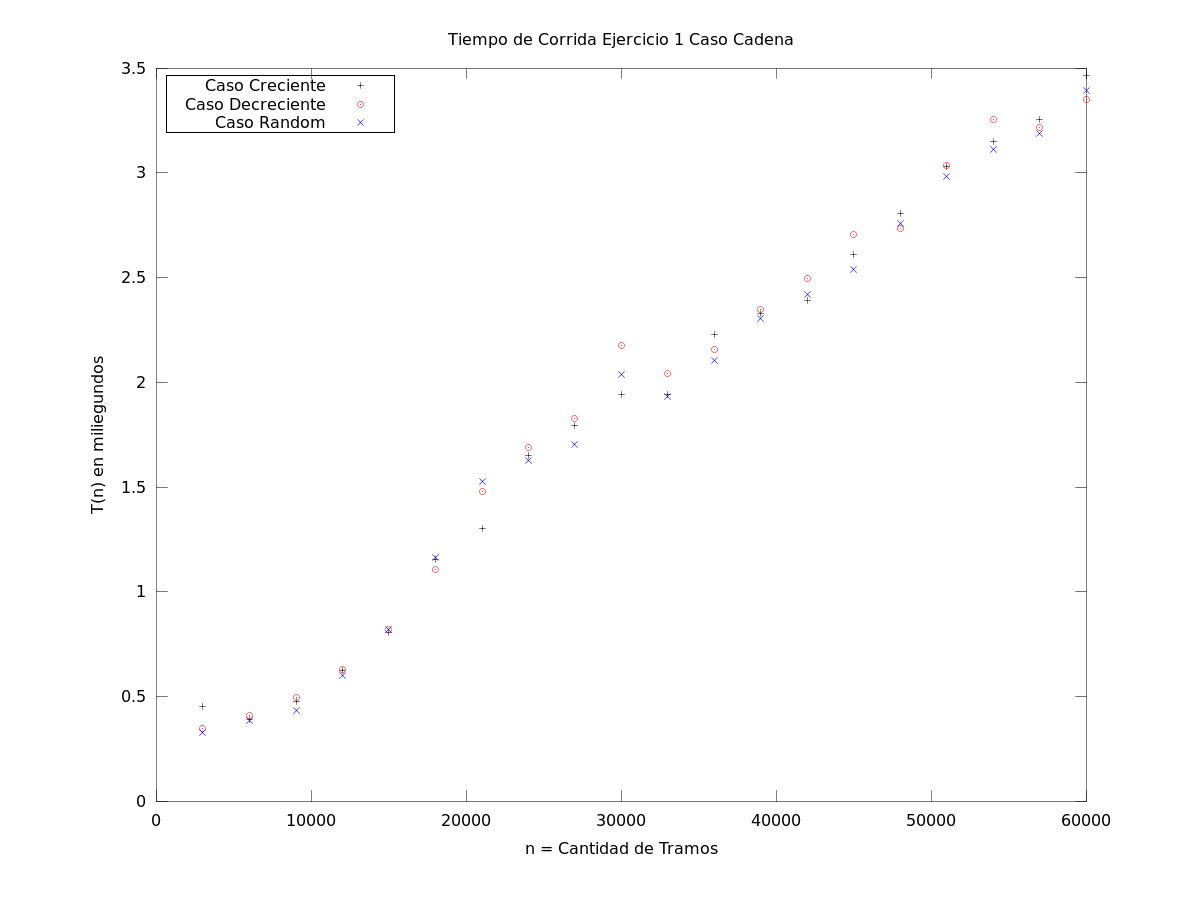
\includegraphics[width=450px]{./figs/cadenas.png}
\end{figure}

\indent Al existir un solo camino que une a la ciudad origen con la ciudad
destino, nuestro algoritmo siempre mantiene un solo elemento en el heap, por lo
que no tiene otra opción mas que tomarlo. Podemos observar que tanto los casos
que tienen números crecientes, como los que tienen números decrecientes, como
también el random, toman tiempos similares. Estos eran los resultados que
esperábamos ya que no importa el valor de los pesos de cada tramo, porque existe
un solo camino a seguir.\\

\clearpage

\textbf{Comparación casos Cadenas Triples}

\begin{figure}[h]
	\centering
	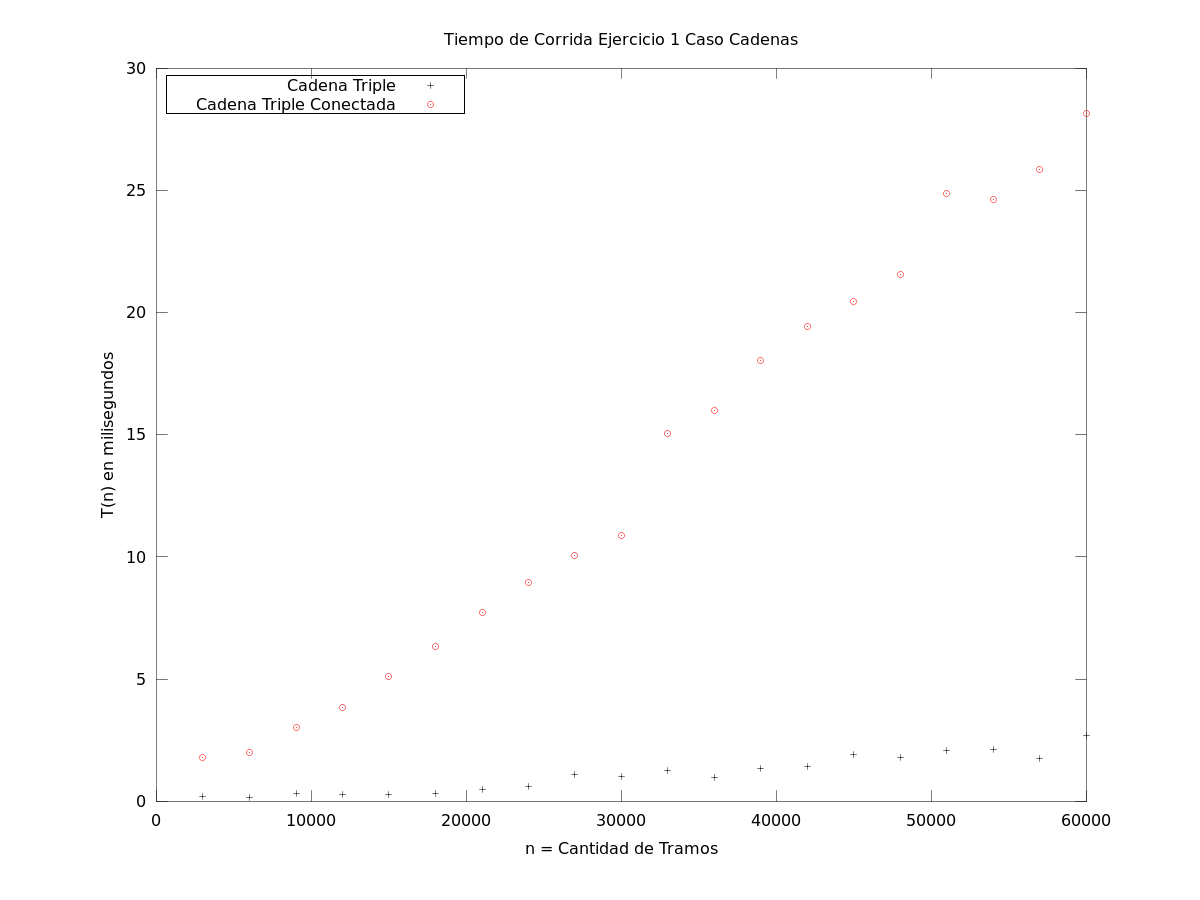
\includegraphics[width=450px]{./figs/cadenasTriples.png}
\end{figure}

\indent La cadena triple conectada tiene mas caminos que llegan al nodo destino,
que la cadena Triple, por lo que el algoritmo evalúa mas posibilidades. Como era
de esperarse, la cadena triple conectada, evalúa muchas mas posibilidades, y es
por eso que su tiempo de corrida es mayor que el de la cadena que solo tiene 3
caminos posibles.\\ 


\clearpage

\textbf{Comparación caso Completo VS Cuadricula}

\begin{figure}[h]
	\centering
	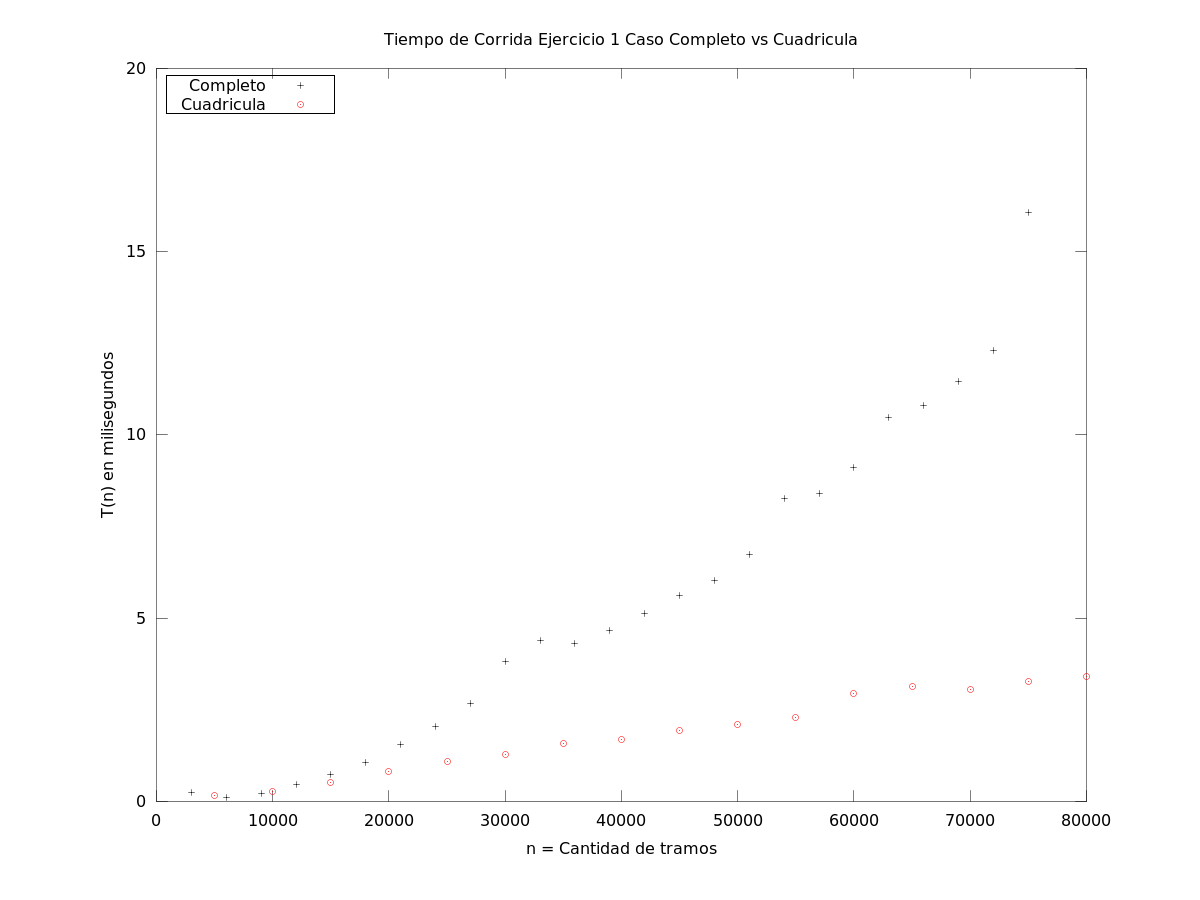
\includegraphics[width=450px]{./figs/completoVScuadricula.png}
\end{figure}

\indent Por como plantemos el caso completo, era de esperarse que tardara mas
que la cuadricula. Esto se da porque nuestro caso completo evalúa todas los
caminos, antes de obtener del heap una de los caminos con peso 1 que llegaba a
la ciudad destino y así terminar la ejecución. 










